\documentclass{beamer}
\usetheme{Singapore}
\usecolortheme{beaver}
\usepackage{subfig}
\usepackage{float}
\graphicspath{{./img/}}



\title{Quasigeostrophic fluids and resonant interactions}
\author{James Hawley}
\date{August 14, 2015}
\institute{University of Waterloo}


\begin{document}

	\begin{frame}
		\titlepage
	\end{frame}

	\section*{Contents}
		\begin{frame}{Contents}
			\tableofcontents
		\end{frame}

	\section{Background}
		\subsection{Hamiltonian Dynamics}
			\begin{frame}[t]{Classical Mechanics}
				\begin{minipage}{0.45\textwidth}
					\begin{itemize}
						\item<2-> Newtonian Dynamics
						\item<3-> $\frac{d^2 \vec q}{dt} = -\nabla \Pi$
						\item<3-> Solve second order system
					\end{itemize}
				\end{minipage}
				\begin{minipage}{0.45\textwidth}
					\begin{itemize}
						\item<4-> Hamiltonian Dynamics
						\item<5-> $\frac{d \vec p}{dt} = -\frac{\partial \mathcal{H}}{\partial \vec q}$
						\item<5-> $\frac{d \vec q}{dt} = \frac{\partial \mathcal{H}}{\partial \vec p}$
						\item<5-> Often first order, coupled system
					\end{itemize}
				\end{minipage}
			\end{frame}
			\begin{frame}[t]{Fluids}
				\begin{minipage}{0.45\textwidth}
					\begin{itemize}
						\item<2-> Navier-Stokes Equations
						\item<3-> $\rho\frac{d \vec u}{dt} = -\nabla p + \rho \nabla \Pi + F$
						\item<3-> Solve system of coupled, non-linear, PDEs
					\end{itemize}
				\end{minipage}
				\begin{minipage}{0.45\textwidth}
					\begin{itemize}
						\item<4-> Hamiltonian
						\item<5-> $\frac{d \vec p}{dt} = -\frac{\partial \mathcal{H}}{\partial \vec q}$
						\item<5-> $\frac{d \vec q}{dt} = \frac{\partial \mathcal{H}}{\partial \vec q}$
					\end{itemize}
				\end{minipage}
			\end{frame}

		\subsection{Shallow Water Model}
			\begin{frame}[t]{Shallow Water Model}
				\begin{center}
					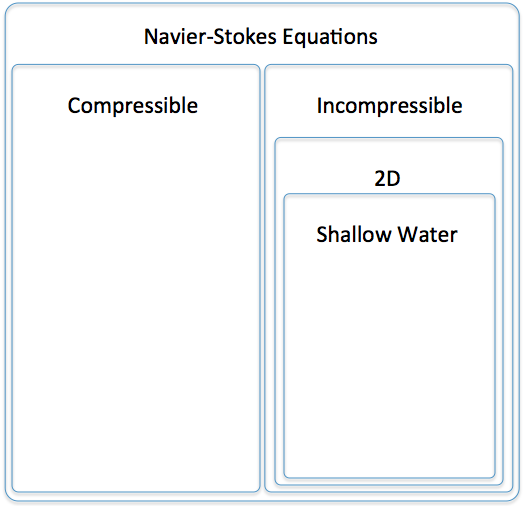
\includegraphics[width=0.4\textwidth]{nested_models_sw.png}
				\end{center}
			\end{frame}
			\begin{frame}[t]{Shallow Water Model}
				\begin{center}
					\begin{minipage}{0.45\textwidth}
						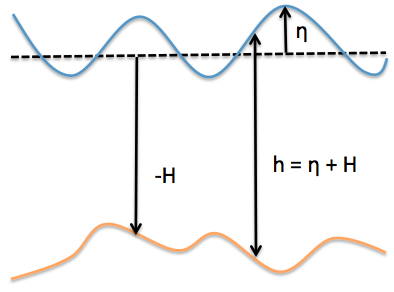
\includegraphics[width=\textwidth]{sw_diagram.png}
					\end{minipage}
					\begin{minipage}{0.45\textwidth}
						\begin{align*}
							0 &=\nabla \cdot \vec u\\
							0 &=\frac{\partial h}{\partial t} + \frac{\partial}{\partial x}(hu) + \frac{\partial}{\partial y}(hv)
						\end{align*}
					\end{minipage}
				\end{center}
			\end{frame}
		\subsection{Quasigeostrophic Model}
			\begin{frame}[t]{Geostrophic Model}
				\begin{center}
					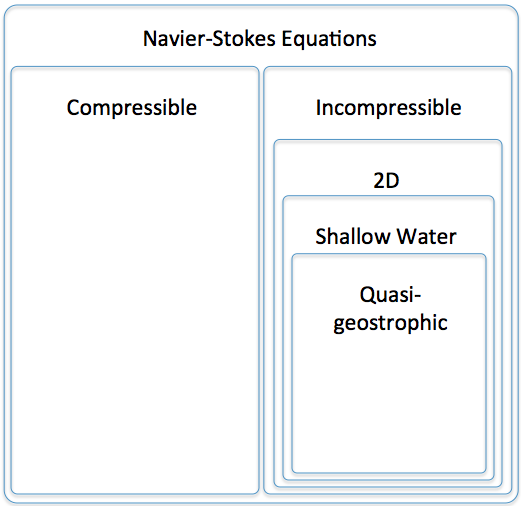
\includegraphics[width=0.4\textwidth]{nested_models_qg.png}
				\end{center}
			\end{frame}
			\begin{frame}[t]{Geostropic Model}
				\begin{align*}
					\frac{d \vec u}{dt} + 2 \vec \Omega \times \vec u &= -\frac{\nabla p}{\rho} + \nabla \Pi + \frac{F}{\rho}\\
					\vec u &= \text{velocity field}\\
					\vec \Omega &= \text{rotation vector}\\
					p &= \text{pressure}\\
					\Pi &= \text{scalar potential field}\\
					F &= \text{viscous forces}\\
				\end{align*}
			\end{frame}
			%--- Next Frame ---%
			\begin{frame}[t]{Quasigeostrophic Model}
				\begin{center}
					\begin{align*}
						0 &=\frac{\partial q}{\partial t} + J(\psi, q) \\
						J(a, b) &=\frac{\partial a}{\partial x}\frac{\partial b}{\partial y} - \frac{\partial a}{\partial y}\frac{\partial b}{\partial x} \\
					\end{align*}
				\end{center}
			\end{frame}

	\section{Main Work}

	\section{References}
		\begin{frame}{References}
			\begin{enumerate}
				\item Reference
			\end{enumerate}
		\end{frame}

\end{document}
